\documentclass{beamer}
%
% Choose how your presentation looks.
%
% For more themes, color themes and font themes, see:
% http://deic.uab.es/~iblanes/beamer_gallery/index_by_theme.html
%
\mode<presentation>
{
  \usetheme{Boadilla}      % or try Darmstadt, Madrid, Warsaw, ...
  \usecolortheme{beaver} % or try albatross, beaver, crane, ...
  \usefonttheme{default}  % or try serif, structurebold, ...
  \setbeamertemplate{navigation symbols}{}
  \setbeamertemplate{caption}[numbered]
  
} 

\usepackage{xcolor,colortbl}
\usepackage[english]{babel}
\usepackage[utf8x]{inputenc}
\usepackage{courier}
\usepackage{dsfont}
\usepackage{verbatim} 
\usepackage{enumerate}
\usepackage{tikz}
\usepackage{multirow}
\usepackage{venndiagram}
\usepackage{epigraph} 
%\usepackage{xcolor}

%\usepackage{enumitem}

\usepackage{hyperref}
\hypersetup{
    colorlinks=true,
    linkcolor=blue,
    filecolor=magenta,      
    urlcolor=cyan,
}

\usetikzlibrary{shapes,decorations,arrows,calc,arrows.meta,fit,positioning}
\tikzset{
    -Latex,auto,node distance =1 cm and 1 cm,semithick,
    state/.style ={ellipse, draw, minimum width = 0.7 cm},
    point/.style = {circle, draw, inner sep=0.04cm,fill,node contents={}},
    bidirected/.style={Latex-Latex,dashed},
    el/.style = {inner sep=2pt, align=left, sloped}
}

\setbeamertemplate{enumerate items}[default]

%\setitemize{label=\usebeamerfont*{itemize item}%
%  \usebeamercolor[fg]{itemize item}
%  \usebeamertemplate{itemize item}}

\newcommand{\Mypm}{\mathbin{\tikz [x=1.4ex,y=1.4ex,line width=.1ex] \draw (0.0,0) -- (1.0,0) (0.5,0.08) -- (0.5,0.92) (0.0,0.5) -- (1.0,0.5);}}%

\title[STA-209]{Data Visualization Part 2}
\subtitle{}
\author{Grinnell College}
\date{September 9, 2024}

\graphicspath{{img/}}

\begin{document}

\begin{frame}
  \titlepage
\end{frame}

\begin{frame}{Review}
We looked at lots of ways to display variables \vspace{4mm}

Some of the graphs we saw:
\begin{itemize}
    \item one categorical variable $\rightarrow$ bar graph
    \item one quantitative variable $\rightarrow$ histogram
    \item categorical + categorical $\rightarrow$ stacked, dodge, conditional bar graph
    \item quantitative + quantitative $\rightarrow$ scatterplot
\end{itemize}
\end{frame}

\begin{frame}{Review}
\fbox{\parbox{4in}{There is an \textbf{association} between variable when knowing about one variable affect what we know about the other}} \vspace{2mm}

ex) We saw that public colleges tend to have higher admission rates \vspace{12mm}

\fbox{\parbox{4in}{The \textbf{distribution} of a variable is a description of how frequently certain values of that variable show up in the data}} \vspace{2mm}
\end{frame}


\begin{frame}{Goals for Today}
We are going to continue to look at ways to visualize data. \vspace{5mm}

At the end of today you will be able to:
\begin{itemize}
    \item describe what a 'percentile' is
    \item explain the parts of a boxplot
    \item recognize what types of graphs to use when we have \hspace{10mm} Categorical + Quantitative variables
\end{itemize}
\end{frame}

\begin{frame}{Percentiles}
A \textbf{percentile} $\alpha$ is a number such that $\alpha\%$ of our (quantitative) observations fall at or below this number when ranked from smallest to largest \vspace{5mm}

Some percentiles have special names. The \textit{median}, for example, is the 50th percentile. \vspace{5mm}

Other notable percentiles include:
\begin{enumerate}
\item Minimum
\item 25th percentile or \textbf{first quartile} ($Q_1$)
\item 75th percentile or \textbf{third quartile} ($Q_3$)
\item Maximum
\end{enumerate}
\vspace{3mm}
\end{frame}

\begin{frame}{IQR}
The \textbf{interquartile range} or \textbf{IQR} is the value of $Q_3 - Q_1$, and gives us the range of the middle 50\% of our data \vspace{3mm}
\end{frame}

\begin{frame}{IQR}
The \textbf{interquartile range} or \textbf{IQR} is the value of $Q_3 - Q_1$, and gives us the range of the middle 50\% of our data \vspace{5mm}

Data: \hspace{2mm} $\{3, 4, 4, 5, 7, 8, 9, 12, 13, 13, 15, 19, 21\}$ \vspace{3mm}

$\{{\color{red}3, 4, 4, 5}, 7, 8, 9, 12, 13, 13, 15, 19, 21\}$ $\rightarrow$ Q1 = 5
$\{{\color{red}3, 4, 4, 5, 7, 8, 9, 12, 13, 13}, 15, 19, 21\}$ $\rightarrow$ Q3 = 13

IQR = Q3 - Q3 = 13 - 5 = 8
\begin{center}
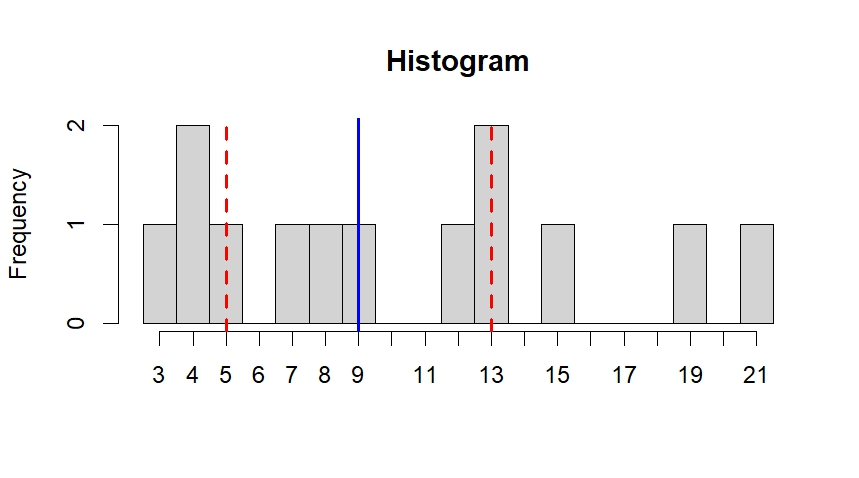
\includegraphics[scale=0.45]{img/IQR_hist.jpeg}
\end{center}
\end{frame}

\begin{frame}{Box plots}
A \textbf{Box plot} is another way to display a quantitative variable, specifically it displays the 5-number-summary \vspace{3mm}

ex) 2019 College data
    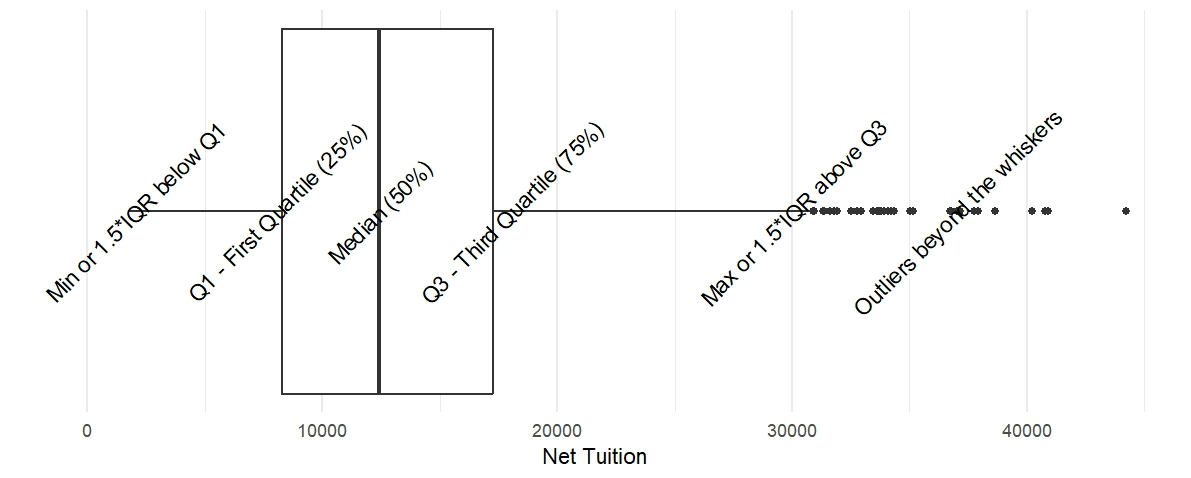
\includegraphics[scale=.55]{img/Boxplot_description.jpeg}
\end{frame}


\begin{frame}{Box plots}
\begin{center}
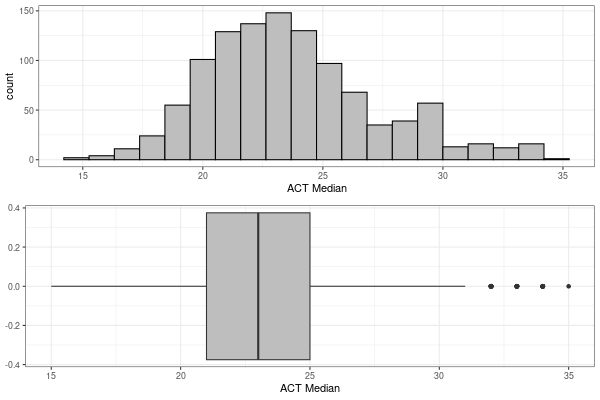
\includegraphics[scale=0.40]{hist_and_box.png}
\end{center}
Using either will (generally) give us the same distribution description
\begin{itemize}
    \item skew is sometimes harder to describe with boxplots
    \item outliers classification is different
\end{itemize}
\end{frame}

\begin{frame}{Box plots}
\begin{center}
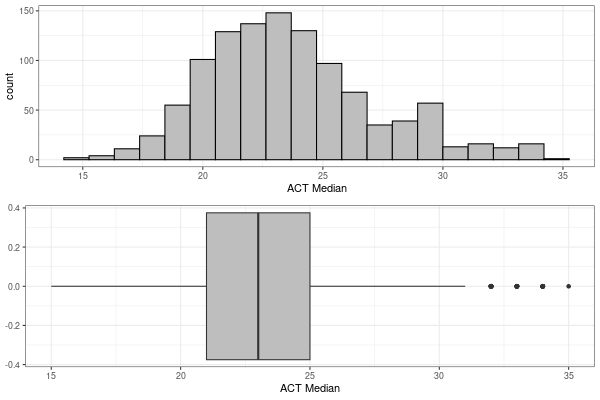
\includegraphics[scale=0.40]{hist_and_box.png}
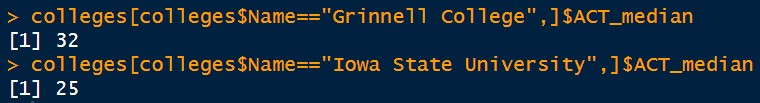
\includegraphics[scale=.5]{img/college_act_example.jpg}
\end{center}
\end{frame}


\begin{frame}{Quantitative + Categorical $\rightarrow$ Side-by-side Box plots}
\begin{center}
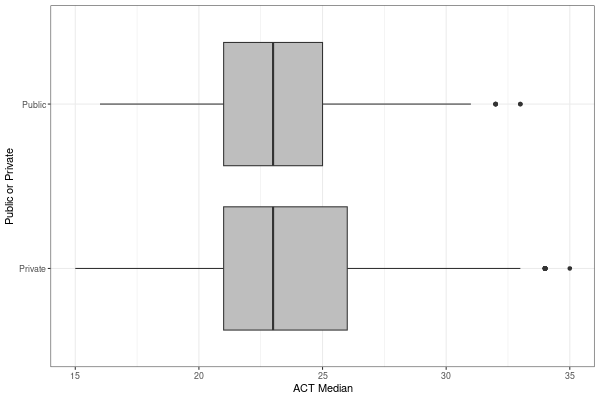
\includegraphics[scale=0.5]{box_private.png}
\end{center}
\end{frame}

\begin{frame}{Quantitative + Categorical $\rightarrow$ Side-by-side Box plots}
\begin{center}
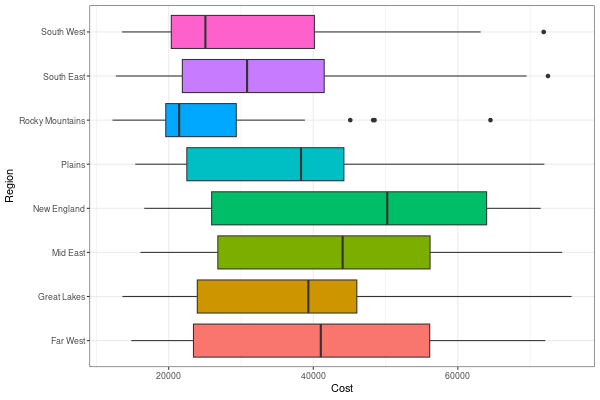
\includegraphics[scale=0.5]{box_private2.png}
\end{center}
\end{frame}

\begin{frame}{Quantitative + Categorical $\rightarrow$ Stacked Histograms}
\begin{columns}
    \begin{column}{0.45\textwidth}
        Instead of doing side-by-side box plots, you may ask why we couldn't do side-by-side (stacked) histograms \vspace{10mm}

        Technically we can, they just get really hard to read and compare
    \end{column}

    \begin{column}{0.45\textwidth}
           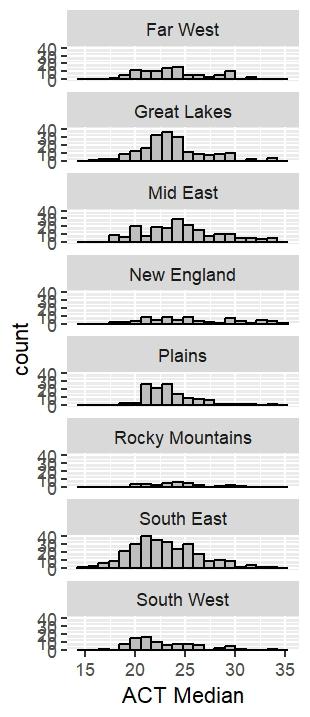
\includegraphics[scale=0.65]{img/stacked_histograms.jpeg}
    \end{column}
\end{columns}
\end{frame}

\begin{frame}{Quantitative + Categorical $\rightarrow$ Grid of Histograms}
\begin{center}
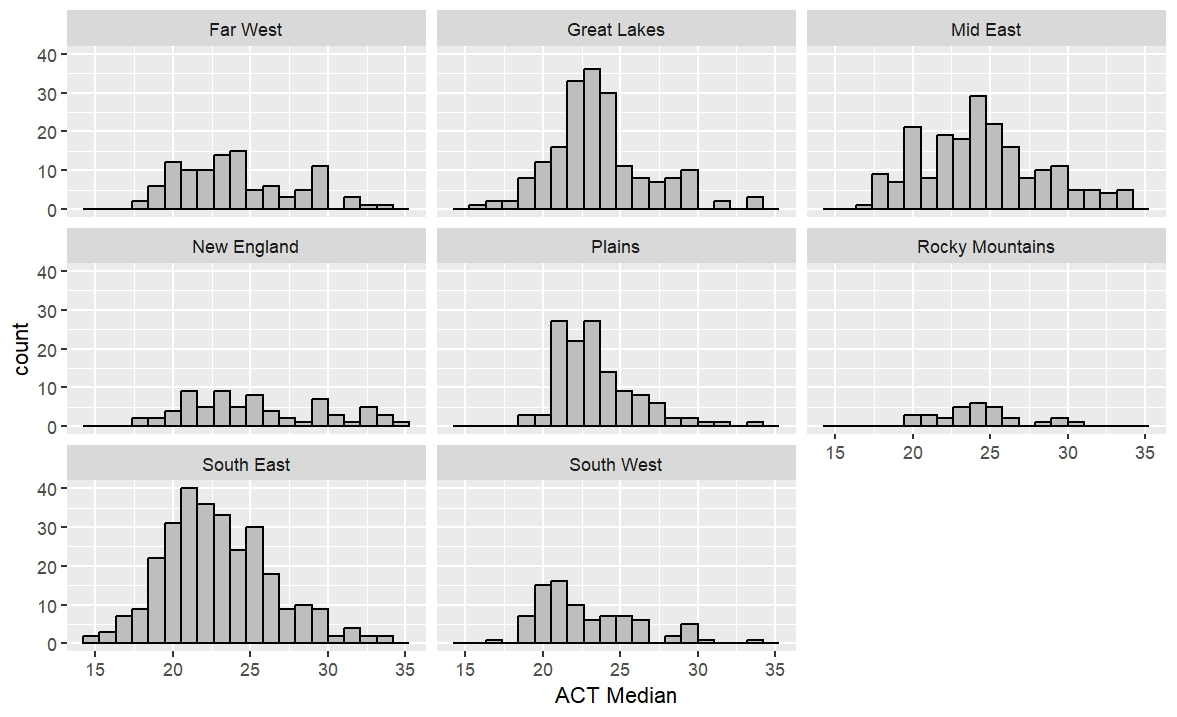
\includegraphics[scale=0.4]{img/histograms_facetwrap.jpeg}
\end{center}

This does not have a special name that I know of... but is another way to display many histograms.
\begin{itemize}
    \item easier to read the individual histograms
    \item still harder to compare each group than if we had just used box plots
\end{itemize}
\end{frame}



\begin{frame}{Even More Variables?!? -- Scatterplot}
\begin{center}
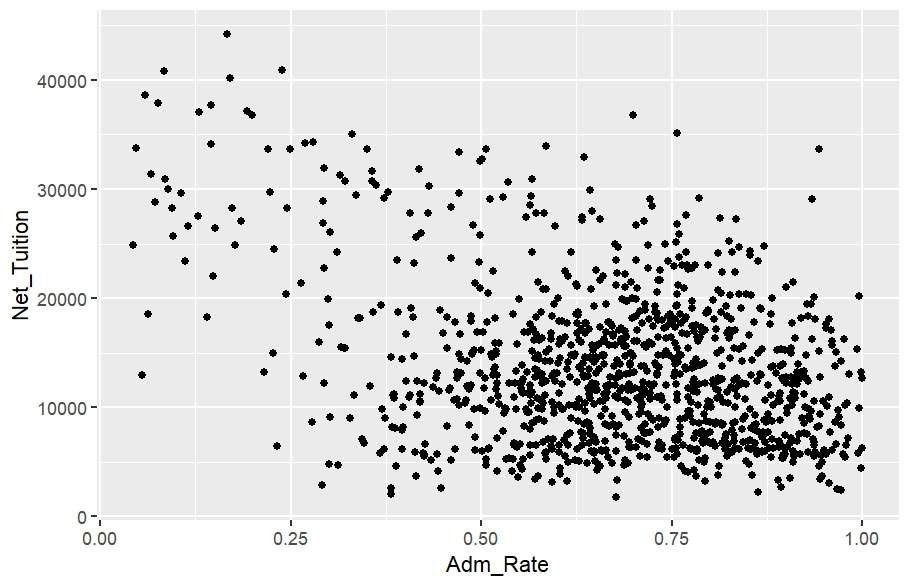
\includegraphics[scale=.7]{img/scatter_example.jpeg}
\end{center}
\end{frame}

\begin{frame}{Even More Variables?!? -- Scatterplot}
\begin{center}
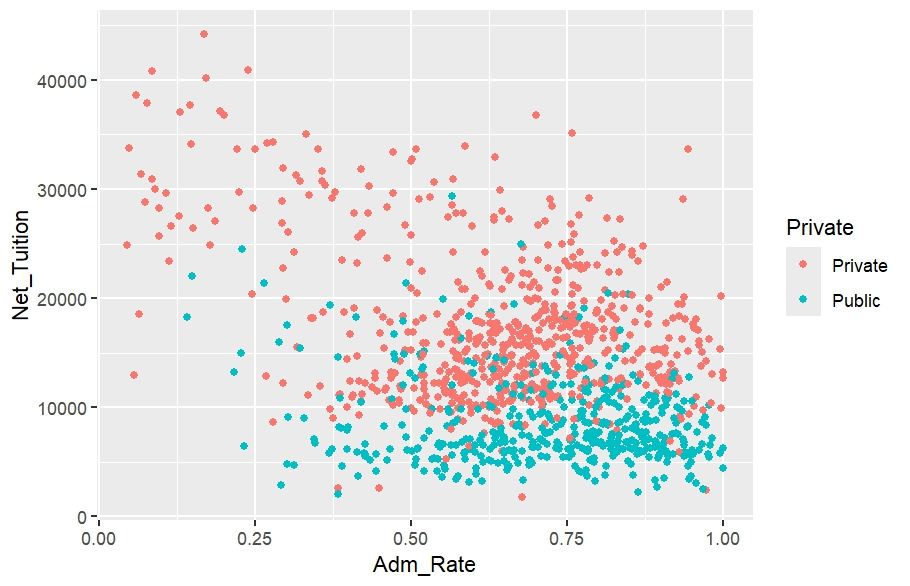
\includegraphics[scale=.7]{img/scatter_by_type.jpeg}
\end{center}
\end{frame}

\begin{frame}{Even More Variables?!? -- Scatterplot}
\begin{center}
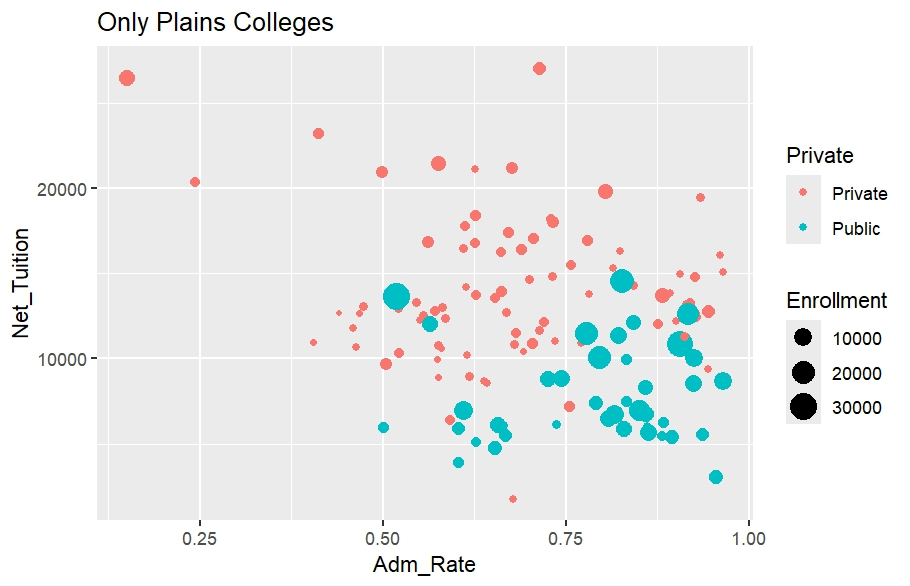
\includegraphics[scale=.7]{img/scatter_by_type_enrollment.jpeg}
\end{center}
\end{frame}


\begin{frame}{Even More Variables?!? -- Scatterplot}
\textbf{BAD EXAMPLE!!}
\begin{center}
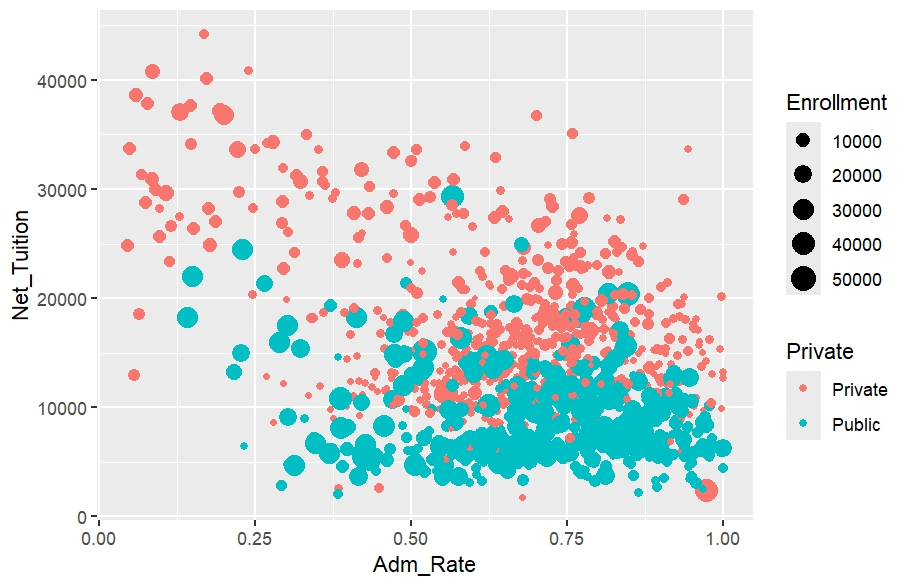
\includegraphics[scale=.7]{img/scatter_by_type_enrollment_all.jpeg}
\end{center}
\end{frame}

\begin{frame}{Even More Variables?!? -- Scatterplot}
\textbf{BAD EXAMPLE!!}
\begin{center}
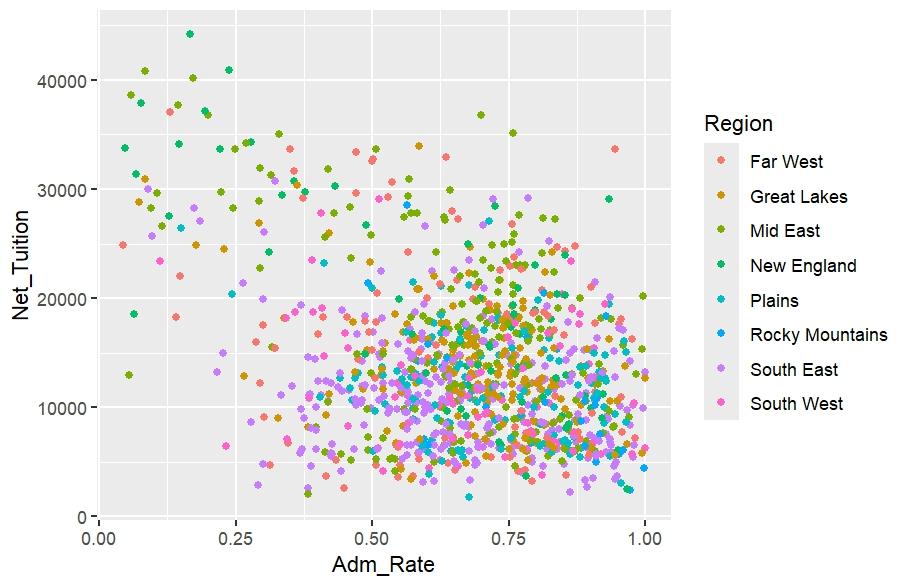
\includegraphics[scale=.7]{img/scatter_by_region.jpeg}
\end{center}
\end{frame}

\begin{frame}{Even More Variables?!? -- Scatterplot}
\textbf{Better?}
\begin{center}
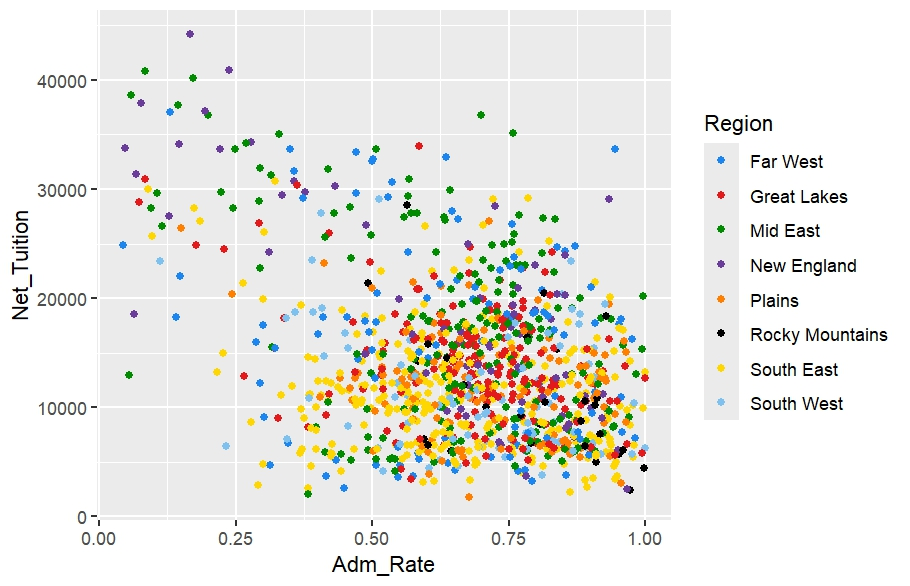
\includegraphics[scale=.7]{img/scatter_by_region2.jpeg}
\end{center}
\end{frame}

\begin{frame}{Review}
\begin{itemize}
\item What is a percentile? \vspace{3mm}
\item What is the IQR, how do we calculate it in terms of Q1 and Q3? \vspace{3mm}
\item Is it easier to compare many groups using side-by-side box plots or histograms?
\end{itemize}
\end{frame}

\begin{frame}{What's Next?}
Today we will work on a lab that puts the data visualization information into practice. \vspace{10mm}

Wednesday we will start looking at how to make pretty graphs using an R package called "ggplot2" \vspace{10mm}

The first homework has been assigned $\rightarrow$ see course page
\begin{itemize}
    \item Similar questions to lab
    \item population, parameter, sample, statistic, observation
    \item data visualization basics
\end{itemize}

\end{frame}



\end{document}


